\section{Experiments}
\label{sec:experiments}

The experiments are designed to evaluate how well SCAPE adapts to different visual scenes, implant layouts, and spatial sampling densities compared to non-adaptive baselines.  
We assess performance across multiple datasets with diverse image statistics and test a range of implant schemes that vary in electrode count and distribution.  
All methods are processed through the same prosthetic vision simulation framework to ensure a fair comparison.  
Performance is quantified using complementary approaches: low-level fidelity metrics applied to phosphene renderings, representational similarity analysis to assess preservation of stimulus relationships, and reconstruction-based evaluation to gauge how well a learned decoder can recover the original scene from each encoding.  
This multi-faceted evaluation allows us to capture both the structural accuracy of the encoded images and their potential usability for downstream perception.


\subsection{Datasets}
We evaluate SCAPE using three publicly available datasets chosen to span complementary domains of visual content and statistics that are relevant for prosthetic vision research:

\begin{itemize}
    \item \textbf{MS~COCO}: diverse natural scenes and everyday objects, providing varied spatial frequencies, textures, and complex layouts. This dataset serves as a benchmark for general-purpose encoding performance in uncontrolled environments.
    \item \textbf{LaPa}: human face images, representing structured, high-contrast features and smooth shading. Faces are particularly important for functional prosthetic vision, since face recognition and interpretation are critical for social interaction.
    \item \textbf{SUN}: indoor and outdoor scene photographs, ranging from cluttered to open environments. This dataset tests how well encoders generalize across large-scale scene structures and semantic diversity, which reflects the types of navigation and recognition tasks prosthesis users encounter in daily life.
\end{itemize}

All images are first converted to grayscale to reflect the fact that brightness is the dominant cue available in prosthetic vision, where phosphenes primarily convey intensity rather than color \cite{Wang2015}.  
In early visual cortex, luminance signals are more strongly represented than chromatic signals, making brightness the most relevant dimension for encoding.  
Preliminary experiments with color confirmed that intensity alone preserved the majority of task-relevant structure.

Grayscale conversion is performed using \textbf{Rec.\,709 perceptual luminance} (luma) weighting, which aligns with human brightness perception:
\begin{equation}
Y = 0.2126\,R + 0.7152\,G + 0.0722\,B,
\end{equation}
where $R$, $G$, and $B$ are normalized to $[0,1]$.  
After conversion, perceptual normalization is applied to ensure a consistent dynamic range across images before encoding.

\begin{table}[ht!]
\centering
\resizebox{\columnwidth}{!}{%
\begin{tabular}{lccc}
\toprule
Scheme & View angle (deg) & Electrodes ($N$) & Eccentricity range (deg) \\
\midrule
Uniform 1024  & 16.0 & 1024 & 0.001--7.984 \\
Neuralink     & 25.0 & 4224 & 0.000--12.095 \\
1 Utah array  & 0.4  & 94   & 0.009--0.203 \\
4 Utah arrays & 16.0 & 320  & 1.632--7.931 \\
\bottomrule
\end{tabular}%
}
\vspace{1em}
\caption{Implant layouts and basic properties. Counts reflect the effective number of electrodes inside the simulator field of view. Eccentricity is reported in degrees of visual angle.}
\label{tab:implant_schemes}
\end{table}


\subsection{Implant Schemes}
We evaluate SCAPE across four implant layouts that span large differences in sampling density, spatial extent, and geometric regularity. This set stresses density adaptation both in the foveal region and in the periphery, and it includes layouts used in recent prosthetic vision studies.

\paragraph{Uniform 1024}
This layout provides a dense, near-uniform sampling of the visual field and serves as a standard reference in the literature on differentiable prosthetic vision. It allows direct comparison to prior work that uses a similar order of magnitude in channel count \cite{deRuytervanSteveninck2020}. It also exposes whether SCAPE preserves fine structure when the density is sufficient across most of the field of view.

\paragraph{Neuralink shank}
This layout represents a high-site-count configuration that covers a wide field of view with thousands of closely spaced sites. Such arrays have been demonstrated in the Neuralink brain–machine interface platform, which integrates flexible polymer shanks with thousands of recording and stimulation channels \cite{Musk2019}. Related developments in ultraflexible electrode arrays further highlight the feasibility of maintaining long-term, high-density interfaces in cortical tissue \cite{Zhao2023}. Within our framework, this scheme stresses computational efficiency and scale selection, since local density varies strongly with eccentricity and along the shank geometry. It therefore provides a test case for whether SCAPE scales robustly to thousands of sites while maintaining stability and efficiency.

\paragraph{One Utah array}
This layout matches a single-array setup and concentrates sampling near fixation with a very small field of view. It reflects ongoing experimental configurations used in current research programs at the Institute of Bioengineering of the Miguel Hernández University. It tests SCAPE under severe channel limits and minimal coverage, which is useful for understanding performance in constrained early clinical or preclinical settings.

\paragraph{Four Utah arrays}
This layout models a realistic multi-array configuration with gaps between arrays and moderate channel count. It introduces strong spatial inhomogeneity due to array borders and inter-array spacing, which is a common feature of practical cortical implants. It therefore tests whether SCAPE can suppress clutter in sparse regions while preserving detail within array footprints.

\begin{figure*}[ht!]
    \centering
    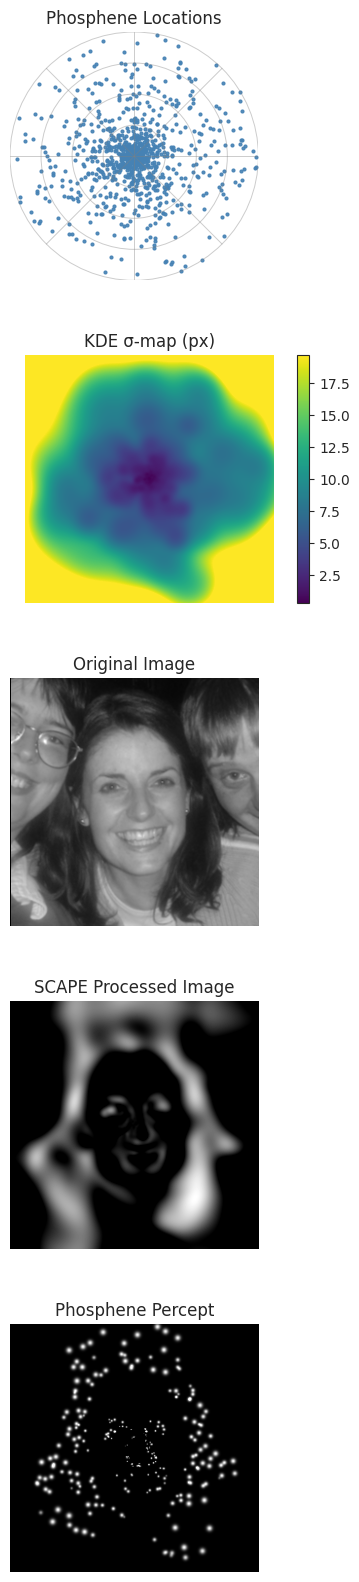
\includegraphics[width=0.23\textwidth]{figures/implant schemes/1024default.png}
    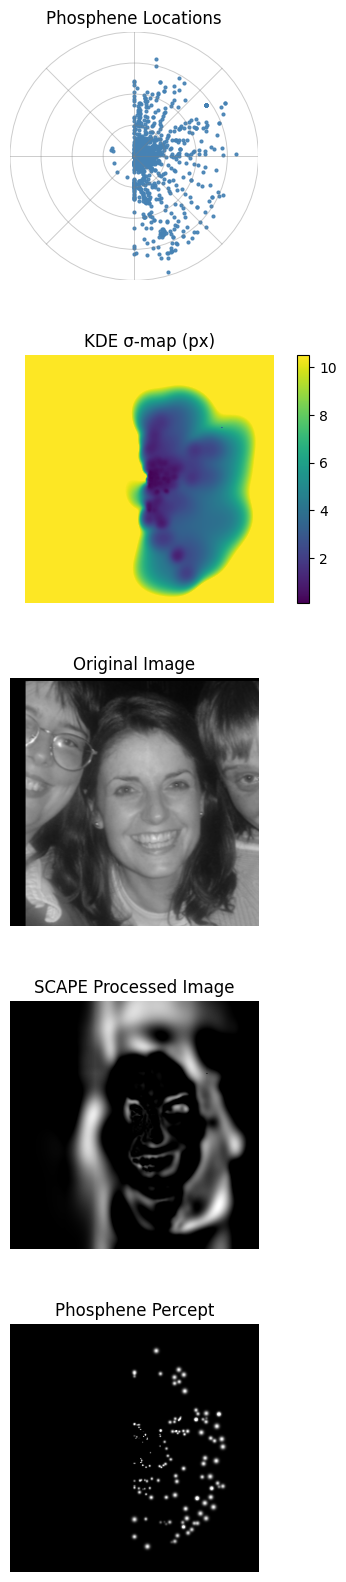
\includegraphics[width=0.223\textwidth]{figures/implant schemes/neuralink.png}
    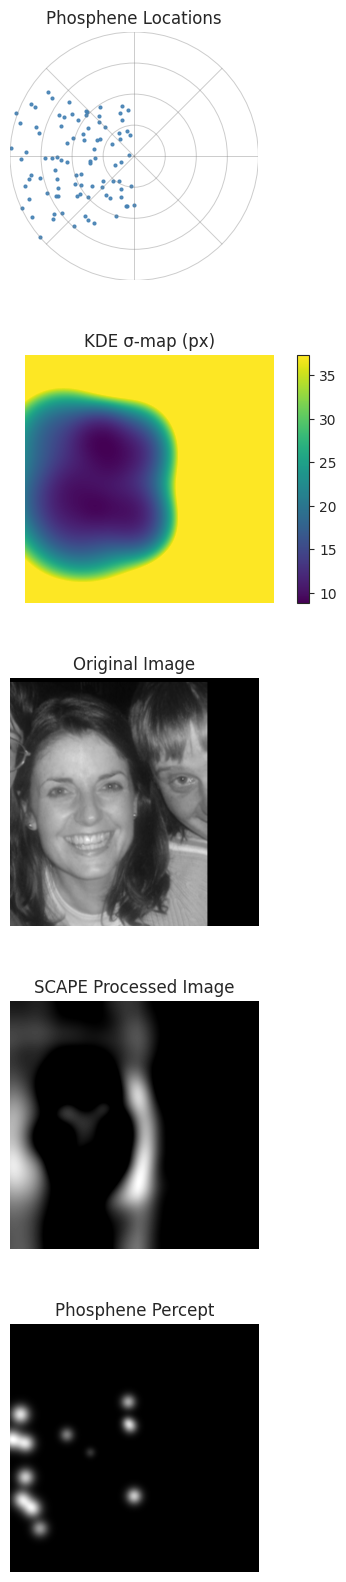
\includegraphics[width=0.223\textwidth]{figures/implant schemes/1 utah array.png}
    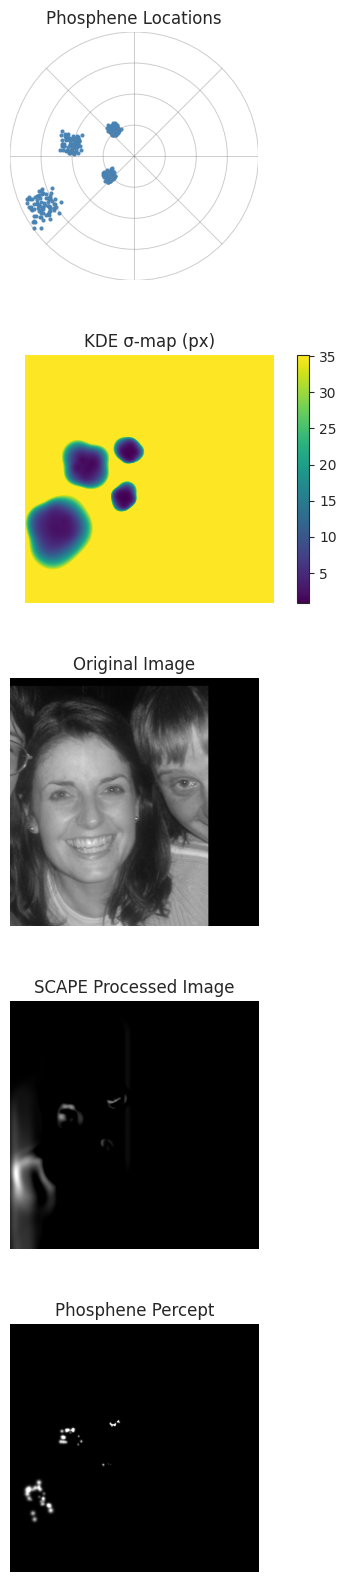
\includegraphics[width=0.223\textwidth]{figures/implant schemes/4 utah arrays.png}
    \caption{\textbf{Implant schemes used for evaluation.} 
    Each column illustrates one of the four electrode layouts tested in this study: Uniform 1024, Neuralink-type shank \cite{Musk2019,Zhao2023}, single Utah array, and four Utah arrays. For each scheme we show (top to bottom): electrode locations in visual field coordinates, the corresponding kernel density estimate (KDE) map of local sampling density, an example input image, the SCAPE-processed representation, and the resulting phosphene percept. The field of view differs between layouts and is scaled here for visualization. Together these schemes span large variations in electrode count, spatial distribution, and coverage, providing a diverse testbed for evaluating adaptive encoding.}
    \label{fig:implant_schemes}
\end{figure*}

\medskip
Together these schemes span two orders of magnitude in channel count, from 94 to 4224. They also span field of view from a fraction of a degree to more than twelve degrees of eccentricity. This diversity is important because SCAPE is designed to set filter scale from local sampling density. The chosen set probes that mechanism in both uniform and highly inhomogeneous layouts, which is essential for a fair test of adaptive encoding.


\subsection{Baselines}
We compare SCAPE against simple, widely used encoding strategies that do not adapt their spatial scale to local sampling density. Each baseline produces an activation map that is passed through the same simulator and amplitude normalization as SCAPE, ensuring that differences in outcome are attributable to the encoding strategy itself.  
Together, these baselines span a spectrum of encoding strategies: a contour-focused method (Canny), a bandpass but nonadaptive method (fixed DoG), and a structure-free random control.

\paragraph{Canny edge detection}
Canny edge maps are a standard choice in prosthetic vision pipelines because they preserve object boundaries under severe spatial resolution limits and often improve recognition in simulated conditions. We include a Canny baseline with standard smoothing and hysteresis thresholding, applied uniformly across the field of view. To enhance the visibility of extracted contours in the simulated percepts, edges are dilated with a $3 \times 3$ kernel \cite{deRuytervanSteveninck2020}. This baseline serves as a strong nonadaptive feature extractor centered on high-contrast contours.

\paragraph{Fixed-scale Difference of Gaussians}
We implement a fixed-scale Difference of Gaussians (DoG) filter as a second baseline. This method applies Gaussian smoothing at a fixed scale and subtracts it from the original image, producing a bandpass representation that emphasizes edges and local contrast. In contrast to SCAPE, the filter scale is uniform across the image and cannot adjust to local variations in sampling density or spatial frequency content. We use a fixed filter size of $\sigma = 3$, chosen to produce feature sizes comparable to the dilated Canny edges.

\paragraph{Random control}
As a structure-free control, we generate a random activation pattern that matches the total activation energy of the method under test. This ensures that any observed improvements are due to meaningful spatial structure in the encoding rather than trivial differences in overall current or luminance.

\begin{figure*}[ht!]
    \centering
    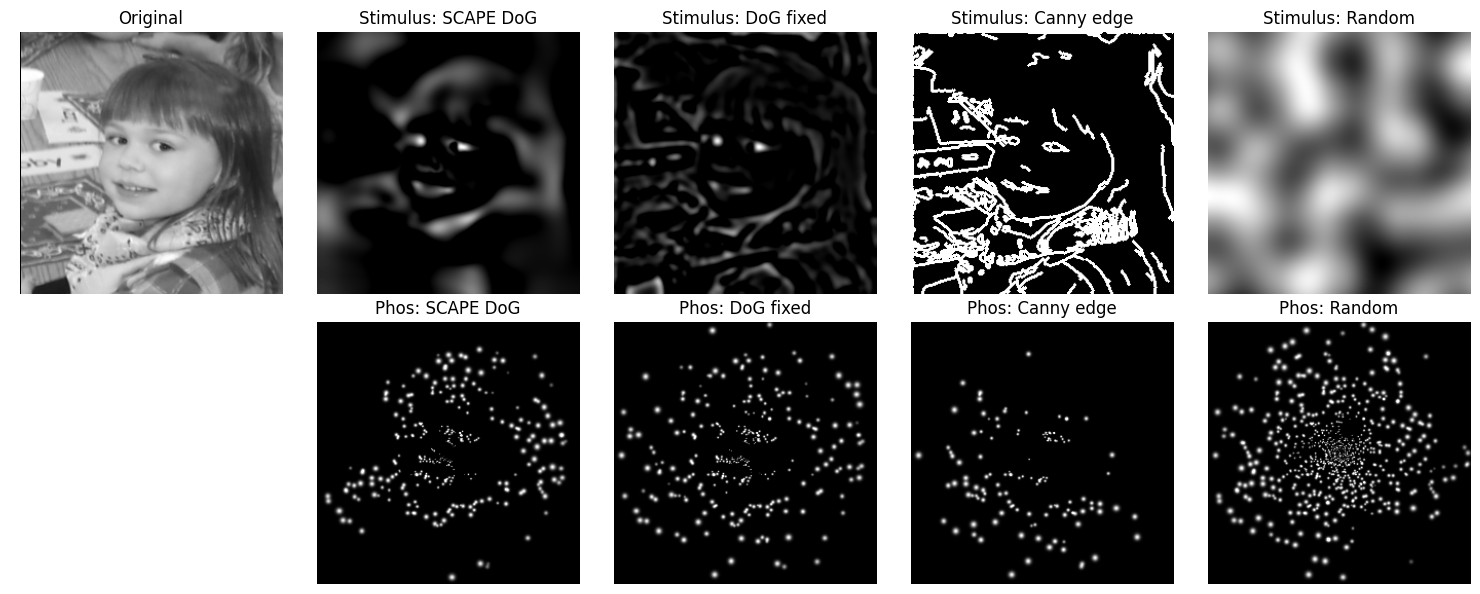
\includegraphics[width=\textwidth]{figures/processingmethods1.png}
    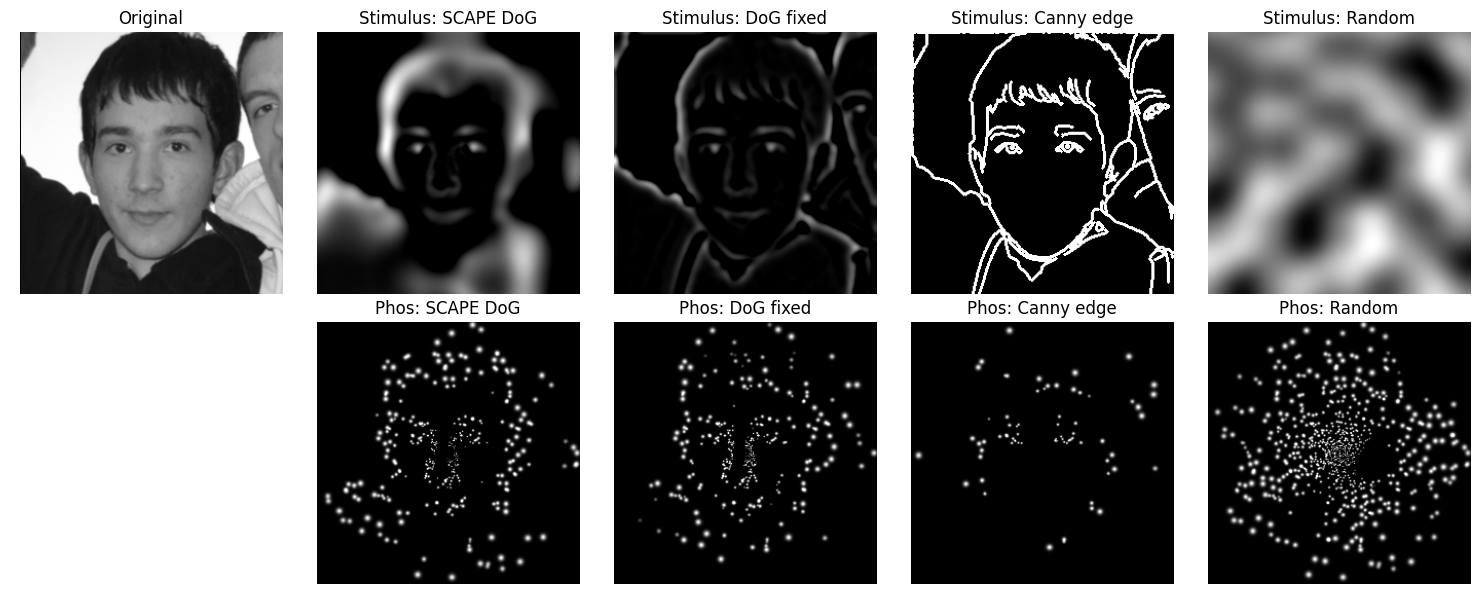
\includegraphics[width=\textwidth]{figures/processingmethods2.png}
    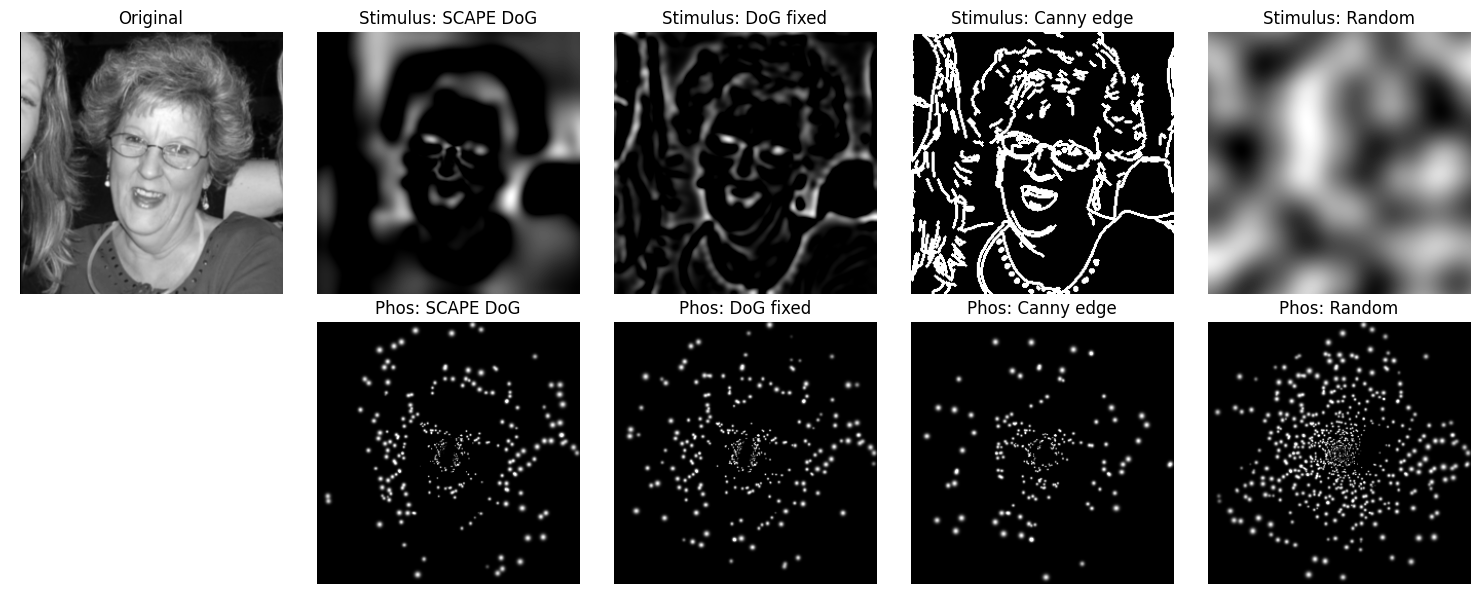
\includegraphics[width=\textwidth]{figures/processingmethods3.png}
    \caption{\textbf{Qualitative comparison of baseline and SCAPE encoders.} 
    Representative examples from the LaPa dataset. Top: stimulus representations after encoding. Bottom: corresponding phosphene renderings for the default implant scheme with 1024 electrodes. 
    SCAPE balances edge emphasis with adaptive clutter suppression, while fixed DoG and Canny either oversmooth or fragment the structure. Random activation patterns are added as a control.}
    \label{fig:qualitative}
\end{figure*}

\medskip
Representative examples of these baselines are shown in Figure~\ref{fig:qualitative}, together with SCAPE for comparison. All methods use identical preprocessing, simulator settings, and amplitude normalization, ensuring that differences in performance reflect only the encoding strategy rather than downstream rendering effects.

\subsection{SCAPE Configuration}
SCAPE builds a local density map from phosphene coordinates using adaptive kernel density estimation and converts that density into a spatial scale map \(\sigma(x,y)\). The scale map controls a shift variant Difference of Gaussians that runs with separable one dimensional passes.

\paragraph{Density estimation}
All experiments use adaptive KDE over phosphene centers in visual field coordinates. Bandwidth \(h_i\) for point \(i\) equals \(\alpha\) times the distance to its \(k\)-th nearest neighbor. We set \(k=16\) and \(\alpha=1.0\). The resulting density map is normalized so that its surface integral equals the total number of phosphenes of the scheme under test.

\paragraph{Mapping density to scale}
We convert density \(d(x,y)\) into a local scale through a Nyquist motivated rule. We use
\[
\sigma_{\text{fov}}(x,y) \;=\; \frac{2}{\pi \sqrt{2}\,\beta}\,\frac{1}{\sqrt{d(x,y)}} \quad\text{with}\quad \beta=0.55,
\]
which yields a scale that decreases in regions with higher sampling density and increases in sparse regions. For filtering on an image grid we convert \(\sigma_{\text{fov}}\) from degrees to pixels using the simulator field of view and resolution.

\paragraph{Stimulus alignment}
To ensure consistency across implant schemes, we center each input stimulus on the centroid of the \(\sigma(x,y)\) map. This alignment guarantees that the most informative regions of the stimulus overlap with the highest density regions of the implant layout, and it standardizes comparisons across schemes.

\paragraph{Filter family and execution}
We use a Difference of Gaussians with ratio \(\lambda=1.6\) to approximate a Laplacian of Gaussian while remaining efficient. The filter runs as two separable Gaussian passes per branch, first horizontal then vertical, at \(\sigma_1(x,y)\) and \(\sigma_2(x,y)=\lambda\,\sigma_1(x,y)\). Gaussian weights are truncated where their value falls below a small threshold and each one dimensional kernel is normalized to sum to one. Padding uses reflection at image borders. The half kernel radius is capped at a fixed maximum to bound runtime and memory.

\paragraph{Retinotopic model}
Retinotopic projection follows the dipole form of the Polimeni wedge–dipole family with standard parameters. This model sets the visual field coordinate system used by the KDE and by the degree to pixel conversion.

\paragraph{Sampling to electrodes}
The shift variant DoG produces an activation map on the simulator grid. Electrode currents are obtained by sampling the activation map at phosphene centers. The same sampling rule is used for every implant scheme.

\subsection{Amplitude Normalization}
To keep comparisons fair across encoders, we apply the same dynamic amplitude equalization to every method. The calibration runs once per implant scheme after mapping activations to electrode currents and before simulation. The resulting per electrode gains are reused for all images and all encoders within that scheme and across datasets. The procedure follows the definition in the Methods section and is tuned for stability.

We optimize the gains with a learning rate of \(0.002\) for \(2000\) steps, constrain each gain to \([0,\texttt{amplitude}]\), and use a small scale factor of \(1\times10^{-4}\) to set the update magnitude. In practice this removes simulator induced brightness bias, reduces extreme responses, and keeps total delivered current comparable, so the results reflect differences in encoding rather than artifacts of the simulation.

\paragraph{Representational similarity analysis}
For each dataset and implant scheme we construct representational dissimilarity matrices (RDMs) for the original images and for each encoded set. 
Each image is converted to a grayscale vector, and pairwise dissimilarity is computed as correlation distance
\[
D_{ij} = 1 - \mathrm{corr}(r_i, r_j).
\]
This produces an RDM that summarizes the relational structure of the stimulus set. 

To compare encoders, we correlate the upper triangular entries of the reference RDM with those of the encoded RDM using Spearman correlation \(\rho\). Higher \(\rho\) indicates closer alignment of relational geometry and thus better preservation of stimulus similarity structure. For visualization, we also report dissimilarity as \(1-\rho\), so that lower values correspond to better preservation. 

To obtain stable estimates, each method is evaluated on 500 randomly sampled images per dataset. Standard errors are estimated by 5000 bootstrap resamples, and statistical significance is assessed with 10{,}000 permutations. We report mean \(\rho\) (and \(1-\rho\) when plotting) per dataset and implant scheme for SCAPE and all baselines.


\paragraph{Reconstruction performance}
We measure how much scene information survives each encoding by training a fixed decoder to reconstruct the original image from phosphene renderings. For every encoder, dataset, and implant scheme we train an Attention U-Net on the corresponding phosphene maps using the same preprocessing, the same simulator settings, and the same training schedule. Inputs and targets are single-channel perceptual luminance images with the normalization described above. Evaluation uses a held-out split and reports MSE, SSIM, PSNR, LPIPS, DISTS, and VSI. Scores are computed per image and summarized as the mean with standard error. We also include representative reconstructions to illustrate qualitative differences that are not fully captured by the metrics.

For practical reasons we restrict reconstruction experiments to the Uniform 1024 scheme. Decoder training is specific to each implant layout, and running it for all schemes would multiply training cost substantially. The 1024 scheme provides a stable, widely used reference case in the literature and offers the fairest setting to compare encoders while keeping evaluation tractable.
